\documentclass[../main.tex]{subfiles}
\begin{document}
\newpage
\lecture{7}{25.02}{}
\begin{proof}
    $\varphi'(t),\psi'(t), \chi'(t) \in C[\alpha,\beta] \implies \exists M>0: |\varphi'(t)|\leqslant M, |\psi'(t)|\leqslant M, |\chi'(t)|\leqslant M \forall t \in [\alpha,\beta].$\\ 
    Берем $\forall T=\{\alpha=t_{0}<t_{1}<\dots<t_{k-1}<t_{k}<\dots<t_{ n}=\beta\}.$ \\По теореме Лагранжа $\exists \alpha_{k},\beta_{k},\gamma_{k}\in (t_{k-1},t_{k}): $
    $\begin{aligned} &\varphi(t_{k})-\varphi(t_{k-1})=\varphi'(\alpha_{k})\Delta t_{k}\\ &\psi(t_{k})-\psi(t_{k-1})=\psi'(\beta_{k})\Delta t_{k}\\ &\chi(t_{k})-\chi(t_{k-1})=\chi'(\gamma_{k})\Delta t_{k}\end{aligned} $ $k=\overline{1,n}$
    $\implies\\\implies l_{T}=\sum_{k=1}^{n} \sqrt{(\varphi(t_{k})-\varphi(t_{k-1}))^{2}+(\psi(t_{k-})-\psi(t_{k-1}))^{2}+(\chi(t_{k})-\chi(t_{k-1}))^{2}} = \sum_{k=1}^{n    } \Delta t_{k}{\sqrt{\underbrace{{(\varphi'(\alpha_{k}))^{2}}+(\psi'(\beta_{k}))^{2}+(\chi(\gamma_{k}))^{2}}_{\leqslant 3M^{2}}}}\leqslant\\\leqslant M\sqrt{3}\sum_{k=1}^{n   } \Delta t_{k}=M \sqrt{3}(\beta-\alpha)\implies\{l_{T}\}-$ ограничена сверху $\implies L-$ спрямляемая. 
    \\ Введем $f(t)=\sqrt{(\varphi(t))^{2}+(\psi(t))^{2}+(\chi(t))^{2}}\in C[\alpha,\beta]\implies f(t) $ интегрируема на $[\alpha,\beta]\implies \exists \int\limits_{\alpha       }^{\beta} f(t)dt=I$, т.е $\underline{\forall \varepsilon>0} \exists \delta_{1}>0: \forall T, \delta_{T}<\delta_{1}, \forall \Xi=\{\xi_{k}\}_{k=1}^{n}\implies |\sigma_{T}(f,\Xi)-I| < \frac{\varepsilon}{2}$ 
    \\$\varphi'(t),\psi'(t),\chi'(t)\in C[\alpha,\beta]\underset{\text{т. Кантора}}{\implies} \varphi'(t),\psi'(t),\chi'(t) - $ равномерно непрерывны на $[\alpha,\beta]\implies \\ \implies \exists \delta_{2}>0 : \forall t',t'' \in [\alpha,\beta] : |t'-t''|<\delta_{2} \implies |\phi'(t')-\varphi'(t'')|<\frac{\varepsilon}{4(\beta-\alpha)}; \; |\psi'(t')-\psi'(t'')|<\frac{\varepsilon}{4(\beta-\alpha)}; \; |\chi'(t')-\chi'(t'')|<\frac{\varepsilon}{4(\beta-\alpha)}.$
    Берем $\delta=\min{(\delta_{1},\delta_{2})}>0, \quad \forall T ,\delta_{T}<\delta, \forall \Xi=\{\xi_{k}\}_{k=1}^{n},$\\ рассмотрим $|l_{T}-I|=|l_{T}-\sigma_{T}(f,\Xi)+\sigma_{T}(f,\Xi)-I| \leqslant |l_{T}-\sigma_{T}(f,\Xi)| + \underbrace{|\sigma_{T}(f,\Xi)-I|}_{<\frac{\varepsilon}{2}}<|l_{T}-\sigma_{T}(f,\Xi)| +\frac{\varepsilon}{2}=\left|\sum_{k=1}^{n} \left[\sqrt{(\varphi'(\alpha_{k}))^{2}+(\psi'(\beta_{k}))^{2}+(\chi'(\gamma_{k}))^{2}}\Delta t_{k}-\sqrt{(\varphi'(\xi_{k}))^{2}+(\psi'(\xi_{k}))^{2}+(\chi'(\xi_{k}))^{2}}\Delta t_{k} \right] \right| + \frac{\varepsilon}{2}\leqslant\\ \leqslant\frac{\varepsilon}{2}+ \sum_{k=1}^{n    } \left| \sqrt{(\varphi'(\alpha_{k}))^{2}+(\psi'(\beta_{k}))^{2}+(\chi'(\gamma_{k}))^{2}} - \sqrt{(\varphi'(\xi_{k}))^{2}+(\psi'(\xi_{k}))^{2}+(\chi'(\xi_{k}))^{2}} \right| \Delta t_{k}\leqslant \\\leqslant\sum_{k=1}^{n    } \sqrt{(\varphi'(\alpha_{k})-\varphi'(\xi_{k}))^{2}+(\psi'(\beta_{k})-\psi'(\xi_{k}))^{2}+(\chi'(\gamma_{k})-\chi'(\xi_{k}))^{2}}\Delta t_{k} +2 < \sum_{k=1}^{n   }\sqrt{\frac{3\varepsilon^{2}}{16(\beta-\alpha)^{2}}}\Delta t_{k} +\frac{\varepsilon}{2}=\\= \frac{\varepsilon\sqrt{3}}{4(\beta-\alpha)}(\beta-\alpha)+\frac{\varepsilon}{2}= \frac{\varepsilon\sqrt{3}}{4}+\frac{\varepsilon}{2}<\frac{\varepsilon}{2}+\frac{\varepsilon}{2}=\varepsilon\implies \lim\limits_{\delta_{T}\to 0} l_{T}=I$ 
    \\ Осталось доказать, что $l_{T}\leqslant I \;\forall T.$ От противного, предположим, что $\exists T_{0}: l_{T_{0}}>I$. Известно, что $\lim\limits_{\delta_{T}\to 0}l_{T}=I,$ т.е $\forall \varepsilon>0 \exists \delta >0: \forall T, \delta_{T}<\delta\implies |l_{T}-I|<\varepsilon.$
    \\ Берем $\varepsilon=\frac{l_{T_{0}}-I}{2}>0 \implies \exists \delta>0 : \forall T ,\delta_{T}<\delta \implies |l_{T}-I| < \frac{l_{T_{0}}-I}{2}$. Берем $T_{1}\succ T_{0} : \delta_{T_{1}}<\delta\implies \frac{l_{T_{0}}-I}{2}=\varepsilon>|l_{T_{1}}-I|=l_{T_{1}}-I \geqslant l_{T_{0}}-I =2\varepsilon\implies$ противоречие $\implies $ предположение неверно $\implies l_{T}\leqslant I \; \forall T$
    
\end{proof}
\newpage
\subsection{Частные случаи гладких кривых:}
1)$y=f(x),x\in[a,b] \quad \begin{cases}
    x=t \\ 
    y=f(t)\\ 
    z\equiv0
\end{cases}t\in[a,b]\implies l(L) = \int\limits_{a  }^{b    } \sqrt{1+(f'(t))^{2}}dt=\int\limits_{a }^{b    } \sqrt{1+(f'(x))^{2}}dx$

 2)$r=r(\varphi), \varphi \in [\alpha,\beta], \quad \begin{cases}
    x=r(\varphi)\cos{\varphi}\\ 
    y=r(\varphi)\sin{\varphi}\\ 
\end{cases}\quad (x'_{\varphi}(\varphi))^{2}+(y'_{\varphi}(\varphi))^{2}=(r'(\varphi)\cos{\varphi}-r(\varphi)\sin{\varphi})^{2}+(r'(\varphi)\sin{\varphi}+r(\varphi)\cos{\varphi})^{2}=r^{2}(\varphi)+(r'(\varphi))^{2}\implies l(L) = \int\limits_{\alpha}^{\beta}\sqrt{r^{2}(\varphi)+(r'(\varphi))^{2}} $
\section{Площадь плоской фигуры. Критерий квадратируемости}
\begin{definition}
    Плоская фигура - любое ограниченное множество на плоскости
\end{definition}
\begin{definition}
    P - плоская фигура. Число $\mu(P)- $ площадь, если: \\
    $\begin{aligned} &1) \mu(P)\geqslant 0
    \\&2) \text{Если фигуры } P_{1} и P_{2} \text{ равны в геометрическом смысле }\implies \mu(P_{1})=\mu(P_{2})
    \\&3)P_{1},P_{2}: P_{1} \cap P_{2} =\varnothing  \implies\mu(P_{1} \cup P_{2})=\mu(P_{1})+\mu(P_{2})
    \\&4) \text{Если } P- \text{ единичный квадрат } \implies \mu(P)=1\end{aligned}$
\end{definition}
\vspace{1cm}
\noindent Объединение, пересечение, вычитание многоугольников - тоже многоугольник. \\$\varnothing  -$ тоже многоугольник ($\mu(\varnothing )=0$). Если $P-$ многоугольник, то его площадь известна ($\tilde{\mu}(P)$ - обозначение площади)

$P$- плоская фигура $\implies Q, S : \underset{вписанный}{Q}\subset P \subset \underset{описанный}{S}$
\\$\forall Q,S : Q\subset P \subset S \implies \tilde{\mu}(Q) \leqslant \tilde{\mu}(S)\implies \{\mu(Q)\}$ - ограничено сверху. $\{\mu(S)\}$ - ограничено снизу.

\begin{definition}
    $ P-$ плоская фигура. $\underline{\mu(P)}=\underset{Q \subset P }{\sup}{\tilde{\mu}(Q)}$ - нижняя площадь. $\overline{\mu(P)}=\underset{S\supset P}{\inf}{\tilde{\mu}(S)}$
\end{definition}

$Q\subset P \subset S \implies \tilde{\mu}(Q)\leqslant \tilde{\mu}(S)\implies \underline{\mu}(P)\leqslant \tilde{\mu}(S)\implies \underline{\mu}(P)\leqslant \overline{\mu}(P)$

\begin{definition}
    Плоская фигура $P$ называется квадрируемой, если $\underline{\mu(P)}=\overline{\mu(P)}.$ При этом $\mu(P)=\underline{\mu(P)}=\overline{\mu(P)}$
\end{definition}

\begin{theorem}
    Введеная таким образом $\mu(P)$ - площадь т.е 
    \\1) $P$ - квадрируемая фигура $\implies \mu (P)\geqslant 0$
    \\2) $P_{1},P_{2}$ - квадрируемые плоские фигуры, причем $P_{1}$ и $P_{2}$ равны в геометрическом смысле $\implies \mu(P_{1})=\mu(P_{2}) $
    \\3) $P_{1},P_{2}$ - квадрируемые плоские фигуры, причем $P_{1} \cap P_{2} = \varnothing \implies P=P_{1}\cup P_{2}$ - тоже квадрируема, причем $\mu(P)=\mu(P_{1})+\mu(P_{2})$
    \\4) Если $P$ - единичный квадрат $\implies P$ - плоская квадрируемая фигура, причем $\mu(P)=1$ 

\end{theorem}


\begin{proof}
    1) $ \exists\mu(P)=\underline{\mu(P)}=\underset{Q\subset P}{\sup}{\underbrace{\tilde{\mu}(P)}_{\geqslant 0}}\geqslant 0$
    \\2)$Q_{1} \subset P_{1} \subset S_{1}\Leftrightarrow Q_{2} \subset P_{2} \subset S_{2},$ причем $Q_{1}$ и $Q_{2}$ равны в геометрическом  смысле, $S_{1}$ и $S_{2}$ равны в геометрическом смысле $\implies \begin{aligned}&\tilde{\mu_{1}}(Q_{1})=\tilde{\mu}(Q_{2}) \\ &\tilde{\mu_{1}}(S_{1})=\tilde{\mu}(S_{2})\end{aligned} \implies \underline{\mu(P_{1})}=\underline{\mu}(P_{2}), \; \overline{\mu}(P_{1})=\overline{  \mu}(P_{2})\implies \mu(P_{1})=\mu(P_{2})$
    \\3) $P_{1}, P_{2}$ - квадрируемые $\implies \exists \mu(P_{1}),\mu (P_{2}),$ причем $\begin{aligned}&\mu(P_{1})= \overline{\mu}(P_{1})= \underline{\mu}(P_{1}) \\ &\mu(P_{2})=\overline{\mu}(P_{2})=\underline{\mu}(P_{2}) \end{aligned}   \implies \forall \varepsilon >0 \exists Q_{1},Q_{2} ,S_{1},S_{2}:\\\begin{aligned} &Q_{1}\subset P_{1}\subset S_{1}: \tilde{\mu}(Q_{1} )>\mu(P_{1}) - \frac{\epsilon}{2}\\ &Q_{2}\subset P_{2} \subset S_{2}:\tilde{\mu}(Q_{2})>\tilde{P_{2}}-\frac{\epsilon}{2}\\ &\phantom{\subset Q_{2} \subset P_{2} \subset S_{2}}\tilde{\mu}(S_{2})< \mu (P_{2})+\frac{\varepsilon}{2} \\ &\phantom{\subset Q_{2} \subset P_{2} \subset S_{2}}\tilde{\mu}{S_{1}}< \mu(P_{1})+\frac{\varepsilon}{2}\end{aligned}$ 
    \\ $Q_{1}\subset P_{1}, Q_{2} \subset P_{2} ,$ но $ P_{1} \cap P_{2}=\varnothing \implies Q_{1} \cap Q_{2} =\varnothing \implies \mu(Q_{1} \cup Q_{2})=\mu(Q_{1})+\mu(Q_{2}),$ причем $\begin{aligned} &Q=Q_{1} \cup Q_{2} \\ &S= S_{1} \cup S_{2} \end{aligned}$
    \\ Рассмотрим $ \mu (Q) = \mu (Q_{1})+ \mu(Q_{2})> \mu(P_{1}) + \mu(P_{2})-\varepsilon.$
    \\ $\underline{\mu}(P)=\underset{Q\subset P}{\tilde{\mu}(Q)}>\underset{\substack{Q: Q_{1} \cup Q_{2} \\ Q_{1} \subset P_{1} \\ Q_{2} \subset P_{2}}}{\sup}{\tilde{\mu}(Q)}\geqslant \tilde{\mu}(Q_{1})+ \tilde{\mu}(Q_{2}) > \mu(P_{1})+ \mu(P_{2})-\varepsilon$ 
    \\ Получили, что $\forall \varepsilon>0 \; \underline(\mu)(P)> \mu(P_{1})+\mu(P_{2})-\varepsilon\implies \underline{\mu}(P)\geqslant \mu(P_{1})+\mu(P_{2})$
    \\ Аналогично: $\tilde{\mu}(S)\leqslant \tilde{\mu}(S_{1})+\tilde{\mu}(S_{2}). \quad \overline{\mu}(P)=\underset{S\supset P}{\inf}{\mu(S)}\leqslant \underset{\substack{S: S_{1}\cup S_{2} \\ S_{1} \supset P_{1}\\S_{2} \supset P_{2}}}{\inf}{\mu(S)}\leqslant \tilde{\mu}(S_{1})+\tilde{\mu}(S_{2})< \mu(P_{1})+\mu(P_{2})+\varepsilon$. 
    \\ Получили, что $ \forall \varepsilon>0 \implies \overline{\mu}(P)<\mu(P_{1})+\mu(P_{2})+\varepsilon\implies \overline{\mu}(P)\leqslant \mu(P_{1})+\mu(P_{2})\implies \mu(P_{1}) +\mu(P_{2})\leqslant \underline{\mu}(P) \leqslant \overline{\mu}(P)\leqslant \mu(P_{1})+\mu(P_{2})\implies \underline{\mu}(P)=\overline{\mu}(P)=\mu(P_{1})+\mu(P_{2})\implies P$ - квадрируема, причем $\mu(P)=\mu(P_{1})+\mu(P_{2})$
    \\4) $P-$ единичный квадрат. Берем $Q,S : Q=P=S\quad \left.\begin{aligned}&\underline{\mu}(P)=\underset{Q \subset P}{\sup}{\tilde{\mu}(Q)}\geqslant 1\\ &\overline{\mu}(P)=\underset{S\supset P}{\inf}{\tilde{\mu}(S)}\end{aligned}\right\} \implies 1\leqslant \underline{\mu}(P )\leqslant \overline{\mu}(P)\leqslant 1 \implies \underline{\mu}(P)=\overline{\mu}(P)=1\implies$ единичный квадрат - плоская квадрируемая фигура, причем $\mu(P)=1$
 \end{proof}
Берем $\forall \varepsilon>0 $
 \begin{center} \scalebox{0.75}{
    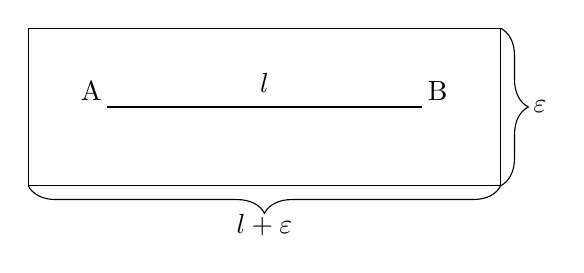
\begin{tikzpicture}
        % Прямоугольник
        \draw (0,0) rectangle (6,2);
    
        % Отрезок внутри прямоугольника
        \draw (1,1) -- (5,1);
    
        % Метки A и B
        \node at (0.8,1.2) {A};
        \node at (5.2,1.2) {B};
    
        % Метка l над отрезком
        \node at (3,1.3) {$l$};
    
        % Скобка для E
        \draw [decorate,decoration={brace,mirror,amplitude=10pt}] (6,0) -- (6,2);
        \node at (6.5,1) {$\varepsilon$};
    
        % Скобка для l + E
        \draw [decorate,decoration={brace,mirror,amplitude=10pt}] (0,0) -- (6,0);
        \node at (3,-0.5) {$l + \varepsilon$};
    \end{tikzpicture}
}
\end{center}
 $\varnothing \subset AB \subset S\qquad 0\leqslant \overline{\mu}(AB)\leqslant \varepsilon(l+\varepsilon)\implies \overline{\mu}(AB)=0; \quad 0\leqslant \underline{\mu}(AB)\leqslant \overline{\mu}(AB)=0\implies \mu(AB)=0$

\vspace{1cm}
\begin{flushright}
    \textit{tg: @moksimqa}
\end{flushright}